\documentclass[a4paper,10pt]{article}

\usepackage{graphicx}
\usepackage{amsmath}
\usepackage[spanish]{babel}
\usepackage[utf8]{inputenc} % Permite escribir directamente áéíóúñ
\usepackage[hidelinks]{hyperref}
\usepackage{pdfpages}

\title{ \textbf{ 6620. Organizaci\'on de Computadoras\\
Trabajo Pr\'actico 2: \\
Programación SIMD, cómputo paralelo y profiling}}

\author{ Riesgo, Daniela, \textit{Padr\'on Nro. 95557} \\
\texttt{ danielap.riesgo@gmail.com } \\[2.5ex]
Martin, D\'ebora, \textit{Padr\'on Nro. 90934} \\
\texttt{ debbie1mes.world@gmail.com } \\[2.5ex]
Constantino, Guillermo, \textit{Padr\'on Nro. 89776} \\
\texttt{ guilleconstantino@gmail.com } \\[2.5ex]
\normalsize{2do. Cuatrimestre de 2014} \\
\normalsize{66.20 Organizaci\'on de Computadoras $-$ Pr\'atica Martes} \\
\normalsize{Facultad de Ingenier\'ia, Universidad de Buenos Aires} \\
}

\date{}

\begin{document}
\maketitle
\thispagestyle{empty} % quita el número en la primer pagina

\newpage
\tableofcontents
\newpage
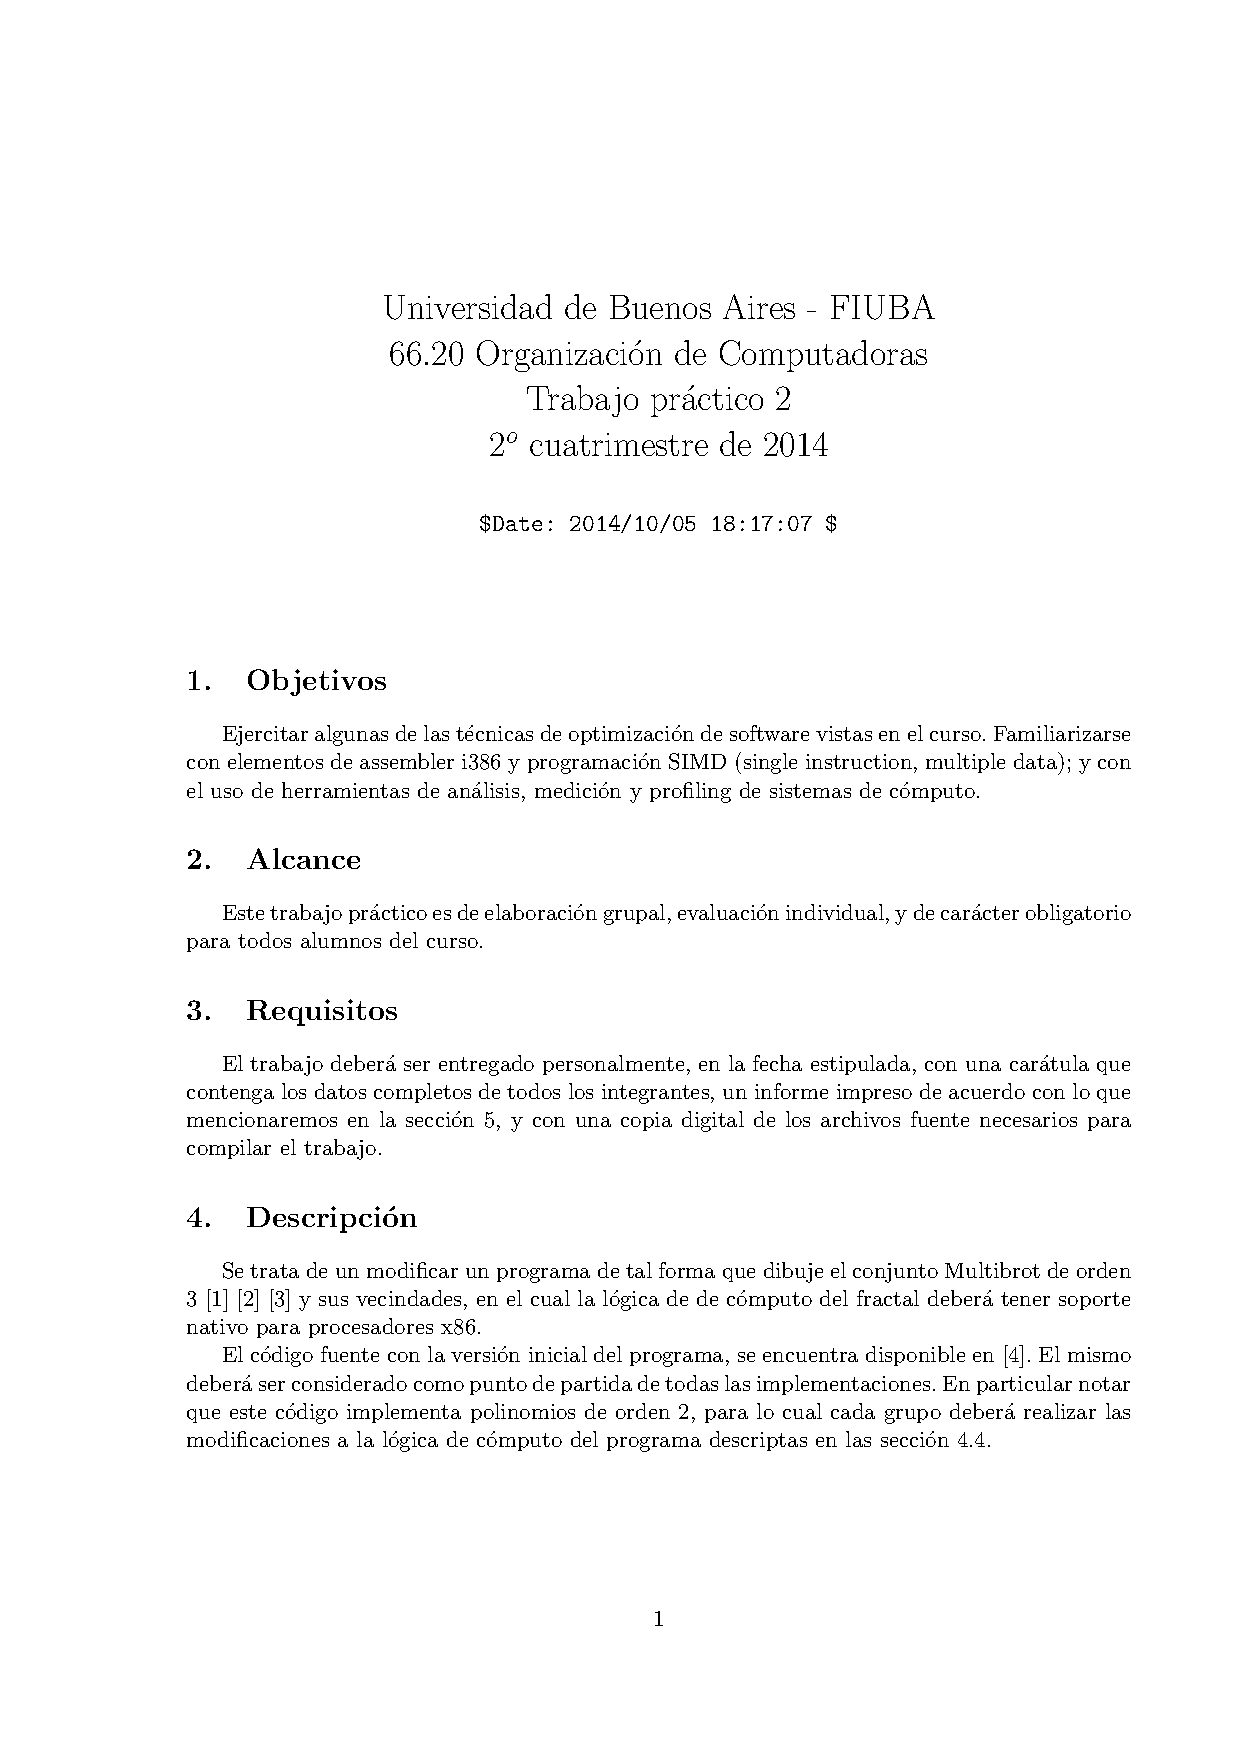
\includepdf[pages={-}]{./Enunciado.pdf}

\begin{abstract}
El presente trabajo tiene como objetivo familiarizarse con assembly x86 SSE mientras se trata con optimizaciones usando programación en paralelo (con $threading$) además de la programación SIMD.

\end{abstract}




\setcounter{page}{2}
\section{Introducci\'on}
Como primer objetivo, nos proponemos adentrarnos en el funcionamiento del assembly x86 SSE y la programación SIMD, en un entorno Intel. Averiguando sobre cómo el procesamiento SIMD permite trabajar con 4 variables flotantes de simple precisión en paralelo y cuáles son las instrucciones que se presentan para manejarlo en entorno Intel, implementándolo desde C con Assembler Inline, que maneja formato AT&T.\\
Luego, aprovechando la programación SIMD y el $threading$ probar distintas formas de procesar la imagen para lograr mejorar el tiempo de ejecución mejorando la parte de plotting de la imagen.




\section{Implementación del programa}

\subsection{Primera parte}
Se trata de alterar el archivo $sse_plot.c$ y el $generic_plot.c$ para graficar el conjunto de Multibrot de orden 3 en vez del conjunto de Mandelbrot que ahora generan.\\
En el archivo $generic_plot.c$ se cambió dentro del ciclo la forma de calcular los nuevos zr y zi. De la misma forma es lo único que debía cambiarse en el $sse_plot.c$. El único inconveniente con este segundo archivo es que los registros no alcanzaban para también recibir un vector de 4 números flotantes de simple precisión que contengan el 3 que debe ser usado en el cálculo de los nuevos zr y zi, pero por suerte podía ser obtenido a partir de restar el vector de 4s y 1's que ya se recibían.\\
Finalmente, para que la región barrida por defecto sea la especificada en el enunciado, también se debieron cambiar los parámetros por defecto del archivo $main.c$ sobre las coordenadas de los puntos del extremo superior izquierdo y el extremo inferior derecho.

\subsection{Segunda parte}
Usando la programación SIMD ya de por si se logra una mejora en tiempo de ejecución ya que se puede procesar 4 pixeles de la imagen a la vez. Sin embargo, la programación con $threading$ puede en ciertos casos mejorar aún más la ejecución, dependiendo de la cantidad de threads a usar y los cores que se tengan disponibles para ejecutarlos.\\
El programa recibido del curso implementa programación en paralelo haciendo threads que se encargan de bandas horizontales de la imagen. Esto no siempre es lo más conveniente porque la imagen puede requerir más cálculo en cierta banda o zona de la imagen que otra.
Por esto primero se decidió probar con procesamiento de bandas verticales de la imagen, esperando que el resultado no fuera tan distinto y dependiera de la zona a dibujar del fractal.
Luego se intentó hacer cómputo paralelo de distintas zonas rectangulares de la imagen, una para cada thread. Nuevamente se espera que dependa de la imagen pero de todas formas se espera un tiempo de cómputo para cada thread equilibrado.

Asique por último se implementó cómputo paralelo en donde se tomara a la imagen como un conjunto de rectángulos y donde cada thread se encargara de calcular varios rectángulos pero que pertenezcan a bandas horizontales y verticales distintas.
COMPLETAAAAR !


Primero, para compilar y obtener el ejecutable del programa se usa la siguiente sentencia:
\begin{verbatim}
$ make -f Makefile.init Makefiles CCARGS="-g -DUSE_SSE_ASSEMBLY -msse"

make -f Makefile.in MAKELEVEL= Makefiles
(echo "# Do not edit -- this file documents how this program was built for your machine."; /bin/sh makedefs) >makedefs.tmp
set +e;                                \
	if cmp makedefs.tmp makedefs.out; then \
	    rm makedefs.tmp;                   \
	else                                   \
	    mv makedefs.tmp makedefs.out;      \
	fi >/dev/null 2>/dev/null
rm -f Makefile; (cat makedefs.out Makefile.in) >Makefile
$ make
\end{verbatim}


Para testear performance se usó el comando time que devuelve el tiempo real, de user y de system. Es decir,
$real$: tiempo desde que se llamó a la función hasta que terminó; esto incluye el tiempo que haya gastado en otros procesos.
$user$: tiempo de CPU que tarda el proceso especificado en modo de usuario y no kernel.
$sys$: tiempo de CPU que tarda el proceso especificado en modo kernel.

Con esto nos importa la parte de cómputo del fractal que es en la cual nos enfocamos en mejorar para obtener un alto SpeedUp por lo que el tiempo $user$ es el que rescataremos de los resultados.

Luego se probó la versión generic y con la función time se obtuvo lo siguiente.
Para estas corridas se utilizaron las versiones 2 de los archivos que corresponden a los mismos archivos de la cátedra pero para el conjunto de Multibrot de orden 3.

\begin{verbatim}
$ time ./tp2-2014-2-bin -o uno.pgm

user	0m0.420s
\end{verbatim}

Con la versión sse se obtuvo:
\begin{verbatim}
$ time ./tp2-2014-2-bin -o uno.pgm -m sse

user	0m0.200s
\end{verbatim}


Si se usan por ejemplo dos threads:
con versión generic
\begin{verbatim}
$ time ./tp2-2014-2-bin -o uno.pgm -n 2

user	0m0.404s
\end{verbatim}

con versión sse
\begin{verbatim}
$ time ./tp2-2014-2-bin -o uno.pgm -m sse -n 2

user	0m0.168s
\end{verbatim}

Pero ya si se usan demasiados threads, esto es contraproductivo al tiempo que le toma al sistema el proceso:
\begin{verbatim}
$ time ./tp2-2014-2-bin -o uno.pgm -m sse -n 10

user	0m0.192s


$ time ./tp2-2014-2-bin -o uno.pgm -m sse -n 20

user	0m0.208s
\end{verbatim}




Más adelante se pensó en probar con bandas verticales en vez de horizontales, esperando que esto dependa de cómo se distribuyan los cálculos en la imagen pero sin poder asegurar nada para cualquier caso general.
Para esto se usó la versión 3 de todos los archivos.

Para 3 threads,
\begin{verbatim}
time ./tp2-2014-2-bin -o uno.pgm -n 3

user	0m0.420s
\end{verbatim}

como el caso visto.
Pero veamos dos nuevas imagénes y comparemos mejor

Versión 3: (Bandas verticales)
\begin{verbatim}
$ time ./tp2-2014-2-bin -o mejor_horizontal.pgm -c -0.5520+0.2001i -n 2

user	0m0.548s


$ time ./tp2-2014-2-bin -o mejor_vertical.pgm -c -0.015+1.2i -H 0.5 -w 0.5 -n 2

user	0m0.348s
\end{verbatim}

Versión 2: (Bandas horizontales)
\begin{verbatim}
$ time ./tp2-2014-2-bin -o mejor_horizontal.pgm -c -0.5520+0.2001i -H 0.5 -w 0.5 -n 2

user	0m0.456s


$ time ./tp2-2014-2-bin -o mejor_vertical.pgm -c -0.015+1.2i -H 0.5 -w 0.5 -n 2

user	0m0.376s
\end{verbatim}

Como se ve, en una imagen en donde lo negro y lo blanco está concentrado en bandas verticales distintas tarda más para esa versión porque se debe esperar a que termine el thread que más tarde en computar (que más negro tenga). Mientras que si lo negro está concentrado en bandas horizontales ese gran cómputo se distribuye en distintos threads disminuyendo el tiempo total. Lo mismo aunque de forma invertida se esperaría en el caso contrario cuando se usa la versión de bandas horizontales, pero las pruebas demuestran lo contrario.
Sin embargo sí podemos decir que el tiempo que tarda en computar el fractal de la imagen mejor_horizontal es mejor en la versión de bandas horizontales que en la de bandas verticales. Y el mismo resultado esperado se da para la otra imagen.



Finalmente se ideó una versión donde la imagen se divida en rectángulos, la cantidad es según especifique el usuario, y se le asigna un thread a cada uno.
Corresponde a la versión 4 de los archivos.


\begin{verbatim}
$ time ./tp2-2014-2-bin -o uno.pgm -m sse
user	0m0.208s

$ time ./tp2-2014-2-bin -o uno.pgm
user	0m0.423s

$ time ./tp2-2014-2-bin -o uno.pgm -m sse -n 2x3
user	0m0.200s

$ time ./tp2-2014-2-bin -o uno.pgm -n 2x3
user	0m0.404s

$ time ./tp2-2014-2-bin -o uno.pgm -m sse -n 3x5
user	0m0.192s

$ time ./tp2-2014-2-bin -o uno.pgm -n 3x5 
user	0m0.440s

$ time ./tp2-2014-2-bin -o uno.pgm -c -0.5520+0.2001i -H 0.5 -w 0.5 -n 2x2
user	0m0.520s

$ time ./tp2-2014-2-bin -o uno.pgm -c -0.015+1.2i -H 0.5 -w 0.5 -n 2x2
user	0m0.364s

\end{verbatim}

Se puede ver como las mejoras no son muy notables, pero sin embargo en comparación con los casos anteriores se ve que esta implementación siempre está dentro de lo aceptable sin ser tener la peor performance pero tampoco la mejor. Esto podemos suponer que se debe a que usa varios threads a la vez y la computadora no puede manejarlos eficientemente.









\section{Corridas de prueba}

Para cada una de las versiones se realizaron las pruebas normales para verificar el funcionamiento correcto.\\

1. Generamos una imagen de 1 punto de lado, centrada en el or\'igen del plano complejo:
\begin{verbatim}
> ./tp0 -c 0+0i -r 1x1 -o -
P2
1
1
255
255
\end{verbatim}

Notar que el resultado es correcto, ya que este punto pertenece al conjunto de Mandelbrot.\\
\\
2. Repetimos el experimento, pero nos centramos ahora en un punto que seguro no pertenece
al conjunto:
\begin{verbatim}
> ./tp0 -c 10+0i -r 1x1 -o -
P2
1
1
255
0
\end{verbatim}

3. Imagen PGM
\begin{verbatim}
> ./tp2-2014-2-bin -o por_default.pgm
\end{verbatim}
Genera la siguiente imagen:
\begin{figure}
\begin{center}

\includegraphics[width=0.8\textwidth]{./por_default.png}
\label{fig:Region barrida por defecto}
\caption{}
\end{center}
\end{figure}


4. Imagen PGM con regi\'on no centrada y un rect\'angulo de 0,005 unidades de lado.
\begin{verbatim}
> ./tp2-2014-2-bin --center -0.6+0.6i --width 0.05 --height 0.05 -o zoom.pgm
\end{verbatim}
Genera la siguiente imagen:
\begin{figure}
\begin{center}

\includegraphics[width=0.8\textwidth]{./zoom.png}
\label{fig:Regi\'on comprendida entre -0.625 + 0.625i y -0.575 + 0.575i.}
\caption{}
\end{center}
\end{figure}


\section{C\'odigo fuente C}
Para cada versión se explicitaran sólo los cambios a partir de los archivos ofrecidos por la cátedra para facilitar la lectura.

\subsection{Versión 2}
\subsubsection{main2.c}
\begin{verbatim}
#include <param2.h>

float upper_left_re = -0.65;	/* Extremo superior izquierzo (re). */
float upper_left_im = +0.30;	/* Extremo superior izquierzo (im). */
float lower_right_re = -0.55;	/* Extremo inferior derecho (re). */
float lower_right_im = +0.20;	/* Extremo inferior derecho (im). */
\end{verbatim}
\subsubsection{generic_plot2.c}
\begin{verbatim}
#include <param2.h>

for (c = 0; c < parms->shades; ++c) {
	if ((absz = zr*zr + zi*zi) >= 4.0f)
		break;
	sr = zr * zr * zr
	   - 3 * zr * zi * zi
	   + cr;
	si = 3 * zr * zr * zi
	   - zi * zi * zi
	   + ci;
	zr = sr;
	zi = si;
}
\end{verbatim}
\subsubsection{sse_plot2.c}
\begin{verbatim}
#include <param2.h>


/* Calculate Z = Z^3 + C. */
"Z_eq_Z3_plus_C:         \n\t"
"movaps   %6, %%xmm6     \n\t" /* xmm6: FOUR */
"subps    %%xmm1, %%xmm6 \n\t" /* xmm6: THREE */

"movaps   %%xmm5, %%xmm7 \n\t" /* xmm7: ZI^2 */
"mulps    %%xmm2, %%xmm7 \n\t" /* xmm7: ZR * ZI^2 */
"mulps    %%xmm6, %%xmm7 \n\t" /* xmm7: 3 * ZR * ZI^2 */
"mulps    %%xmm4, %%xmm2 \n\t" /* xmm2: ZR^3 */
"subps    %%xmm7, %%xmm2 \n\t" /* xmm2: ZR^3 - 3 * ZR * ZI^2 */

"mulps    %%xmm4, %%xmm6 \n\t" /* xmm6: 3 * ZR^2 */
"mulps    %%xmm3, %%xmm6 \n\t" /* xmm6: 3 * ZR^2 * ZI */
"mulps    %%xmm3, %%xmm5 \n\t" /* xmm5: ZI^3 */
"subps    %%xmm5, %%xmm6 \n\t" /* xmm6:  3 * ZR^2 * ZI - ZI^3 */

"addps    %3, %%xmm2     \n\t" /* xmm2: += CR */
"addps    %4, %%xmm6     \n\t" /* xmm6: += CI */
							   /* xmm2: new ZR */
"movaps   %%xmm6, %%xmm3 \n\t" /* xmm3: new ZI */

"jmp      loop           \n\t"
\end{verbatim}


\subsection{Versión 3}
\subsubsection{main3.c}
\begin{verbatim}
#include <param3.h>

float upper_left_re = -0.65;	/* Extremo superior izquierzo (re). */
float upper_left_im = +0.30;	/* Extremo superior izquierzo (im). */
float lower_right_re = -0.55;	/* Extremo inferior derecho (re). */
float lower_right_im = +0.20;	/* Extremo inferior derecho (im). */

parms.x0 = 0;
parms.x1 = x_res;
size_t x0 = 0;
size_t xd = x_res / nthreads;

for (tn = 0; tn < nthreads; ++tn) {
	memcpy(&tinfo[tn].parms, &parms, SZ(parms));
	tinfo[tn].parms.x0 = x0;
	tinfo[tn].parms.x1 = (tn < (nthreads - 1))
	                     ? (x0 = x0 + xd)
	                     : (x_res);

	if (pthread_create(&tinfo[tn].tid, 
	                   NULL, 
	                   (void *)plot,
	                   &tinfo[tn].parms) != 0) {
		fprintf(stderr, "cannot create thread.\n");
		exit(1);
	}
}

\end{verbatim}
\subsubsection{param3.h}
\begin{verbatim}
typedef struct {
	float UL_re;
	float UL_im;
	float LR_re;
	float LR_im;
	float d_re;
	float d_im;

	size_t x_res;
	size_t y_res;
	size_t shades;

	size_t x0;
	size_t x1;

	uint8_t *bitmap;
} param_t;
\end{verbatim}

\subsubsection{generic_plot3.c}
\begin{verbatim}
#include <param3.h>

ci = parms->UL_im;
u8 = parms->bitmap + parms->x0;

for (y = 0; y < parms->y_res; ++y) {
	cr = parms->UL_re + parms->x0 * parms->d_re; 

	for (x = parms->x0; x < parms->x1; ++x) {
		
		zr = cr;
		zi = ci;

		/*
		 * Determinamos el nivel de brillo asociado al punto
		 * (cr, ci), usando la fórmula compleja recurrente 
		 * f = f^3 + c.
		 */
		for (c = 0; c < parms->shades; ++c) {
			if ((absz = zr*zr + zi*zi) >= 4.0f)
				break;
			sr = zr * zr * zr
			   - 3 * zr * zi * zi
			   + cr;
			si = 3 * zr * zr * zi
			   - zi * zi * zi
			   + ci;
			zr = sr;
			zi = si;
		}

		/* Escribimos la intensidad del px. */
		*u8++ = (uint8_t)c;

		/* Calculamos la siguiente parte real. */
		cr += parms->d_re;
	}
	/* Calculamos el lugar en el bitmap de la proxima linea. */
	u8 += (parms->x_res - (parms->x1 - parms->x0));

	/* Calculamos la siguiente parte compleja. */
	ci -= parms->d_im;
	
}

\end{verbatim}
\subsubsection{sse_plot3.c}
\begin{verbatim}
#include <param3.h>

CR0[0] = parms->UL_re + (parms->x0 + 0.5f) * parms->d_re;
CR0[1] = parms->UL_re + (parms->x0 + 1.5f) * parms->d_re;
CR0[2] = parms->UL_re + (parms->x0 + 2.5f) * parms->d_re;
CR0[3] = parms->UL_re + (parms->x0 + 3.5f) * parms->d_re;
INIT4(CI0, parms->UL_im - 0.5f * parms->d_im);

u8 =  parms->bitmap + parms->x0;

/* Calculate Z = Z^3 + C. */
"Z_eq_Z3_plus_C:         \n\t"
"movaps   %6, %%xmm6     \n\t" /* xmm6: FOUR */
"subps    %%xmm1, %%xmm6 \n\t" /* xmm6: THREE */

"movaps   %%xmm5, %%xmm7 \n\t" /* xmm7: ZI^2 */
"mulps    %%xmm2, %%xmm7 \n\t" /* xmm7: ZR * ZI^2 */
"mulps    %%xmm6, %%xmm7 \n\t" /* xmm7: 3 * ZR * ZI^2 */
"mulps    %%xmm4, %%xmm2 \n\t" /* xmm2: ZR^3 */
"subps    %%xmm7, %%xmm2 \n\t" /* xmm2: ZR^3 - 3 * ZR * ZI^2 */

"mulps    %%xmm4, %%xmm6 \n\t" /* xmm6: 3 * ZR^2 */
"mulps    %%xmm3, %%xmm6 \n\t" /* xmm6: 3 * ZR^2 * ZI */
"mulps    %%xmm3, %%xmm5 \n\t" /* xmm5: ZI^3 */
"subps    %%xmm5, %%xmm6 \n\t" /* xmm6:  3 * ZR^2 * ZI - ZI^3 */

"addps    %3, %%xmm2     \n\t" /* xmm2: += CR */
"addps    %4, %%xmm6     \n\t" /* xmm6: += CI */
							   /* xmm2: new ZR */
"movaps   %%xmm6, %%xmm3 \n\t" /* xmm3: new ZI */

"jmp      loop           \n\t"



size_t suma_u8 = parms->x_res - (parms->x1 - parms->x0);
		
__asm__ volatile (
	"U8_avanza_una_linea:    \n\t"
#if _LP64
	"addq     %2, %0         \n\t"
#else
	"addl     %2, %0         \n\t"
#endif		
	: "=r" (u8)		/* %0 */
	: "0" (u8),		/* %1 */
	  "m" (suma_u8)/* %2 */
	: "cc"
);

\end{verbatim}

\subsection{Versión 4}
\subsubsection{main4.c}
\begin{verbatim}
#include <param4.h>

float upper_left_re = -0.65;	/* Extremo superior izquierzo (re). */
float upper_left_im = +0.30;	/* Extremo superior izquierzo (im). */
float lower_right_re = -0.55;	/* Extremo inferior derecho (re). */
float lower_right_im = +0.20;	/* Extremo inferior derecho (im). */
size_t nthreads_x = 1;            /* Cantidad de threads de cómputo en x. */
size_t nthreads_y = 1;            /* Cantidad de threads de cómputo en y. */

static void
do_nthreads(const char *name, const char *spec)
{
	int nt_x, nt_y;
	char x, c;

	if (sscanf(spec, "%d%c%d %c", &nt_x, &x, &nt_y, &c) != 3 
		|| nt_x <= 0 || nt_y <= 0 || x != 'x')
	do_usage(name, 1);

	/* Set new threads. */
	nthreads_x = nt_x;
	nthreads_y = nt_y;
}

size_t y0, x0;
size_t yd, xd;
size_t tn, nt;

parms.y0 = 0;
parms.y1 = y_res;
parms.x0 = 0;
parms.x1 = x_res;

if ((tinfo = malloc(SZ(struct thread_info) * nthreads_x * nthreads_y)) == NULL) {
	fprintf(stderr, "cannot allocate memory.\n");
	exit(1);
}

y0 = 0;
yd = y_res / nthreads_y;
x0 = 0;
xd = x_res / nthreads_x;

for (tn = 0; tn < nthreads_y; ++tn) {
	for (nt = 0; nt < nthreads_x; ++nt){
		memcpy(&tinfo[tn * nthreads_x + nt].parms, &parms, SZ(parms));
		tinfo[tn * nthreads_x + nt].parms.y0 = y0 + tn * yd ;
		tinfo[tn * nthreads_x + nt].parms.y1 = tn < (nthreads_y - 1)
							 ? (y0 + (tn + 1) * yd)
							 : (y_res);
		tinfo[tn * nthreads_x + nt].parms.x0 = x0 + nt * xd;
		tinfo[tn * nthreads_x + nt].parms.x1 = nt < (nthreads_x - 1)
							 ? (x0 + (nt + 1) * xd)
							 : (x_res);
							 
		if (pthread_create(&tinfo[tn * nthreads_x + nt].tid, 
						   NULL, 
						   (void *)plot,
						   &tinfo[tn * nthreads_x + nt].parms) != 0) {
			fprintf(stderr, "cannot create thread.\n");
			exit(1);
		}
	}
}




\end{verbatim}
\subsubsection{param4.h}
\begin{verbatim}
typedef struct {
	float UL_re;
	float UL_im;
	float LR_re;
	float LR_im;
	float d_re;
	float d_im;

	size_t x_res;
	size_t y_res;
	size_t shades;

	size_t y0;
	size_t y1;
	size_t x0;
	size_t x1;

	uint8_t* bitmap;
} param_t;
\end{verbatim}

\subsubsection{generic_plot4.c}
\begin{verbatim}
#include <param4.h>

ci = parms->UL_im - parms->y0 * parms->d_im;
u8 = parms->bitmap + parms->y0 * parms->x_res + parms->x0;

for (y = parms->y0; y < parms->y1; ++y) {
	cr = parms->UL_re + parms->x0 * parms->d_re;

	for (x = parms->x0; x < parms->x1; ++x) {
		zr = cr;
		zi = ci;

		/*
		 * Determinamos el nivel de brillo asociado al punto
		 * (cr, ci), usando la fórmula compleja recurrente 
		 * f = f^3 + c.
		 */
		for (c = 0; c < parms->shades; ++c) {
			if ((absz = zr*zr + zi*zi) >= 4.0f)
				break;
			sr = zr * zr * zr
			   - 3 * zr * zi * zi
			   + cr;
			si = 3 * zr * zr * zi
			   - zi * zi * zi
			   + ci;
			zr = sr;
			zi = si;
		}

		/* Escribimos la intensidad del px. */
		*u8++ = (uint8_t)c;

		/* Calculamos la siguiente parte real. */
		cr += parms->d_re;
	}
	/* Calculamos el lugar en el bitmap de la proxima linea. */
	u8 += (parms->x_res - (parms->x1 - parms->x0));

	/* Calculamos la siguiente parte compleja. */
	ci -= parms->d_im;
}

\end{verbatim}
\subsubsection{sse_plot4.c}
\begin{verbatim}
#include <param4.h>

CR0[0] = parms->UL_re + (parms->x0 + 0.5f) * parms->d_re;
CR0[1] = parms->UL_re + (parms->x0 + 1.5f) * parms->d_re;
CR0[2] = parms->UL_re + (parms->x0 + 2.5f) * parms->d_re;
CR0[3] = parms->UL_re + (parms->x0 + 3.5f) * parms->d_re;
INIT4(CI0, parms->UL_im - (parms->y0 + 0.5f) * parms->d_im);

u8 = parms->bitmap + parms->y0 * parms->x_res + parms->x0;

/* Calculate Z = Z^3 + C. */
"Z_eq_Z3_plus_C:         \n\t"
"movaps   %6, %%xmm6     \n\t" /* xmm6: FOUR */
"subps    %%xmm1, %%xmm6 \n\t" /* xmm6: THREE */

"movaps   %%xmm5, %%xmm7 \n\t" /* xmm7: ZI^2 */
"mulps    %%xmm2, %%xmm7 \n\t" /* xmm7: ZR * ZI^2 */
"mulps    %%xmm6, %%xmm7 \n\t" /* xmm7: 3 * ZR * ZI^2 */
"mulps    %%xmm4, %%xmm2 \n\t" /* xmm2: ZR^3 */
"subps    %%xmm7, %%xmm2 \n\t" /* xmm2: ZR^3 - 3 * ZR * ZI^2 */

"mulps    %%xmm4, %%xmm6 \n\t" /* xmm6: 3 * ZR^2 */
"mulps    %%xmm3, %%xmm6 \n\t" /* xmm6: 3 * ZR^2 * ZI */
"mulps    %%xmm3, %%xmm5 \n\t" /* xmm5: ZI^3 */
"subps    %%xmm5, %%xmm6 \n\t" /* xmm6:  3 * ZR^2 * ZI - ZI^3 */

"addps    %3, %%xmm2     \n\t" /* xmm2: += CR */
"addps    %4, %%xmm6     \n\t" /* xmm6: += CI */
							   /* xmm2: new ZR */
"movaps   %%xmm6, %%xmm3 \n\t" /* xmm3: new ZI */

"jmp      loop           \n\t"


size_t suma_u8 = parms->x_res - (parms->x1 - parms->x0);
		
__asm__ volatile (
	"U8_avanza_una_linea:    \n\t"
#if _LP64
	"addq     %2, %0         \n\t"
#else
	"addl     %2, %0         \n\t"
#endif		
	: "=r" (u8)		/* %0 */
	: "0" (u8),		/* %1 */
	  "m" (suma_u8)/* %2 */
	: "cc"
);


\end{verbatim}

\pagebreak


\section{Conclusiones}


\pagebreak

\begin{thebibliography}{99}

\bibitem{GXEMUL} GXemul, \url{http://gxemul.sourceforge.net/}

\bibitem{NETBSD} The NetBSD Project, \url{http://www.netbsd.org/}

\bibitem{MANDEL} Mandelbrot, \url{http://en.wikipedia.org/wiki/Mandelbrot\_set/}

\bibitem{MANSET} Introduction to the Mandelbrot Set,
\url{http://www.olympus.net/personal/dewey/mandelbrot.html}.

\bibitem{MANEXT} Smooth shading for the Mandelbrot exterior.
\url{http://linas.org/art-gallery/escape/smooth.html}. Linas Vepstas. October, 1997.

\bibitem{PGMFORMAT} PGM format specification.
\url{http://netpbm.sourceforge.net/doc/pgm.html}

\bibitem{LATEX} Oetiker, Tobias, "The Not So Short Introduction To LaTeX2", \url{http://www.physics.udel.edu/$\sim$dubois/lshort2e/}

\end{thebibliography}


\end{document}
